\section{Results}
\begin{figure}[h!]
	\centering
	\includegraphics[width=1\linewidth, keepaspectratio]{tech_comp.eps}
	\caption{}
	\label{fig:tech-comp}
\end{figure}%
%
\subsection{Comparing data extraction techniques}
In figure \ref{fig:tech-comp} three different q-EELS maps are plotted for the radial, linear and slicing technique from top to bottom respectively. It is immediately obvious that the radial and linear "integration" techniques have higher resolutions along the momentum transfer axis. This is due to the fact that slicing the EFTEM stack between two points yields a pixelated line, similarly to opening paint and drawing a line, whereas the integration techniques extract information from pixel just besides the line between two points giving smaller momentum transfer steps. One drawback to these techniques is that they also add intensity values from pixels not directly between to diffraction spots to the q-EELS map, this is especially so with the radial integration technique that uses all values on a circle outwards from the starting point.
The integration techniques also yield a smoother gradient from low-$q_{\perp}$ to high-$q_{\perp}$ since it averages multiple q-EELS spectra in a ringsize, this again might introduce spectra not truly on the line in between two points but does average out any unwanted errors such as external radiation.\\
\newpage%
%
\begin{figure}[h!]
	\centering
	\includegraphics[width=1\linewidth, keepaspectratio]{qmap_corr_comp.eps}
	\caption{Batson correction for qmap}
	\label{fig:bat-cor}
\end{figure}
%
\subsection{Reviewing Batson correction}



\subsection{Interesting features from data}

\begin{figure}
	\centering
	\includegraphics[width=1\linewidth, keepaspectratio]{qmap_peak.eps}
	\caption{tracked peaks on stitched qmap}
	\label{fig:qmap-track}
\end{figure}


\begin{figure}
	\centering
	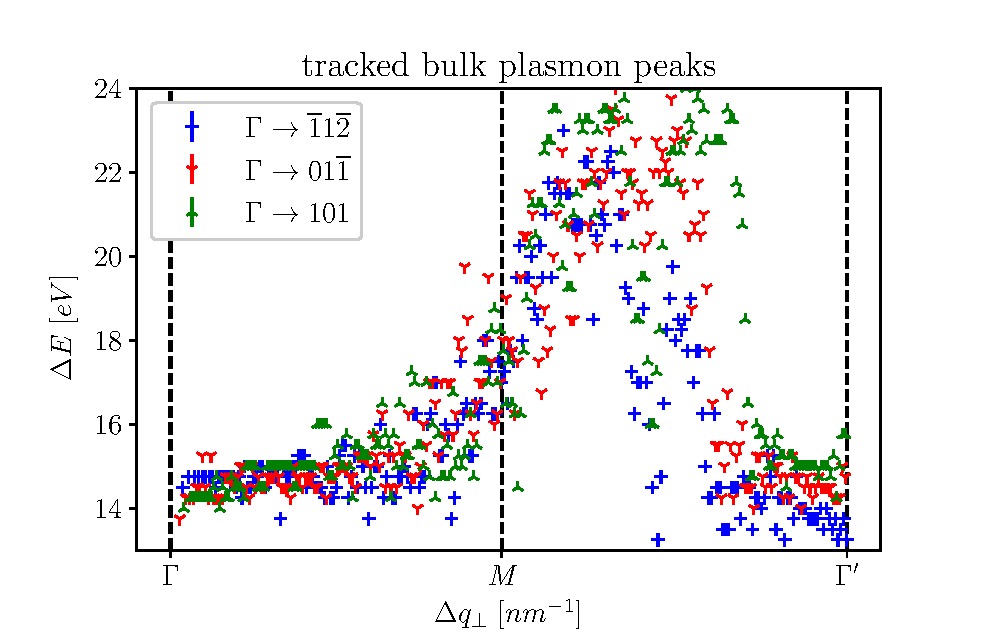
\includegraphics[width=0.5\linewidth, keepaspectratio]{plasmon_dispersion.eps}
	\caption{Tracked peaks of the plasmon dispersion.}
	\label{fig:plas_disp}
\end{figure}

\begin{figure}
	\centering
	\includegraphics[width=0.5\linewidth, keepaspectratio]{track_peak.eps}
	\caption{Tracked peaks of the plasmon dispersion.}
	\label{fig:track_peak}
\end{figure}